\documentclass[a4paper,12pt]{extarticle}

\usepackage[utf8x]{inputenc}
\usepackage[T1,T2A]{fontenc}
\usepackage[russian]{babel}
\usepackage{hyperref}
\usepackage{indentfirst}
\usepackage{listings}
\usepackage{color}
\usepackage{here}
\usepackage{array}
\usepackage{multirow}
\usepackage{graphicx}
\usepackage{caption}
\usepackage{subcaption}
\usepackage{chngcntr}
\usepackage{amsmath}
\usepackage{amssymb}
\usepackage{pgfplots}
\usepackage{pgfplotstable}
\renewcommand{\lstlistingname}{Программа} % заголовок листингов кода

\bibliographystyle{ugost2008ls}

\usepackage{listings}
\lstset{ %
extendedchars=\true,
keepspaces=true,
language=C++,						% choose the language of the code
basicstyle=\scriptsize,		% the size of the fonts that are used for the code
numbers=left,					% where to put the line-numbers
numberstyle=\scriptsize,		% the size of the fonts that are used for the line-numbers
stepnumber=1,					% the step between two line-numbers. If it is 1 each line will be numbered
numbersep=5pt,					% how far the line-numbers are from the code
backgroundcolor=\color{white},	% choose the background color. You must add \usepackage{color}
showspaces=false				% show spaces adding particular underscores
showstringspaces=false,			% underline spaces within strings
showtabs=false,					% show tabs within strings adding particular underscores
frame=single,           		% adds a frame around the code
tabsize=2,						% sets default tabsize to 2 spaces
captionpos=t,					% sets the caption-position to top
breaklines=true,				% sets automatic line breaking
breakatwhitespace=false,		% sets if automatic breaks should only happen at whitespace
escapeinside={\%*}{*)},			% if you want to add a comment within your code
postbreak=\raisebox{0ex}[0ex][0ex]{\ensuremath{\color{red}\hookrightarrow\space}},
texcl=true,
inputpath=fig,                     % директория с листингами
}

\usepackage[left=2cm,right=2cm,
top=2cm,bottom=2cm,bindingoffset=0cm]{geometry}

%% Нумерация картинок по секциям
\usepackage{chngcntr}
\counterwithin{figure}{section}
\counterwithin{table}{section}

%%Точки нумерации заголовков
\usepackage{titlesec}
\titlelabel{\thetitle.\quad}
\usepackage[dotinlabels]{titletoc}

%% Оформления подписи рисунка
\addto\captionsrussian{\renewcommand{\figurename}{Рисунок}}
\captionsetup[figure]{labelsep = period}

%% Подпись таблицы
\DeclareCaptionFormat{hfillstart}{\hfill#1#2#3\par}
\captionsetup[table]{format=hfillstart,labelsep=newline,justification=centering,skip=-10pt,textfont=bf}

%% Путь к каталогу с рисунками
\graphicspath{{fig/}}


\begin{document}	% начало документа

% Титульная страница
\begin{titlepage}	% начало титульной страницы

	\begin{center}		% выравнивание по центру

		\large Санкт-Петербургский Политехнический Университет Петра Великого\\
		\large Институт компьютерных наук и технологий \\
		\large Кафедра компьютерных систем и программных технологий\\[6cm]
		% название института, затем отступ 6см
		
		\huge Вычислительная математика\\[0.5cm] % название работы, затем отступ 0,5см
		\large Отчет по лабораторной работе №1\\[0.1cm]
		\large <<Сравнение точности интерполяционных полиномов>>\\[0.1cm]
		\large Вариант №5\\[5cm]

	\end{center}


	\begin{flushright} % выравнивание по правому краю
		\begin{minipage}{0.25\textwidth} % врезка в половину ширины текста
			\begin{flushleft} % выровнять её содержимое по левому краю

				\large\textbf{Работу выполнил:}\\
				\large Ламтев А.Ю.\\
				\large {Группа:} 23501/4\\
				
				\large \textbf{Преподаватель:}\\
				\large Цыган В.Н.

			\end{flushleft}
		\end{minipage}
	\end{flushright}
	
	\vfill % заполнить всё доступное ниже пространство

	\begin{center}
	\large Санкт-Петербург\\
	\large \the\year % вывести дату
	\end{center} % закончить выравнивание по центру

\thispagestyle{empty} % не нумеровать страницу
\end{titlepage} % конец титульной страницы

\vfill % заполнить всё доступное ниже пространство


\section{Цель работы}
Численно решить систему дифференциальных уравнений.

\section{Решаемые задачи}
\begin{enumerate}

\item Привести дифференциальное уравнение второго порядка

\begin{displaymath}
	t(t+1)y'' + (3t+2)y'  + y = 0
\end{displaymath}

к системе двух дифференциальных уравнений первого порядка.


	Начальные условия: $\left.y \right|_{t=1} = 1$, $\left.y' \right|_{t=1} = -1$, $t \in[1, 2]$  

    Точное решение: $y(t)=\frac{1}{t}$	
		


\item Решить с шагом $h = 0.1$

\begin{enumerate}[label=\arabic*)]
\item Используя RKF45
\item Используя метод Эйлера-Коши
\end{enumerate}

\item Сравнить результаты полученные двумя методами с точным решением.

\end{enumerate}


\section{Ход выполнения работы}

В ходе выполнения работы было разработано программное обеспечение на языке программирования \textbf{java}, позволяющее решить поставленные задачи. Данное программное обеспечение включает в себя:
\begin{itemize}

\item Библиотеку \textbf{MatrixUtil} с функциями \textbf{decomp} и \textbf{solve}, которые содержат вызовы стандартных форсайтовских функций \textbf{decomp} и \textbf{solve}, разработанных на языке программирования \textbf{с}, из динамической библиотеки.

\item Библиотеку \textbf{Matrix}, позволяющую совершать различные действия над матрицами, в том числе, \textit{обращение, произведение, вычитание, вычисление нормы}, которые необходимы для решения поставленных задач.

 \textit{Обращение} матрицы реализовано как n итераций решения системы $\textbf{A}x = \textbf{B}$ при помощи функций \textbf{decomp} и \textbf{solve} c $\textbf{B}$ -- i-м столбцом единичной матрицы на i-й итерации и n -- порядком матрицы. Реализация представлена в листинге \ref{code:Matrix:inverted}.
 
 Реализации \textit{произведения, вычитания, вычисления нормы} представлены в листингах \ref{code:Matrix:multiply}, \ref{code:Matrix:minus} и \ref{code:Matrix:calculateNormAsMaximumAbsoluteColumnSum} соответственно.

\item Приложение, решающее поставленные задачи и использующее ранее перечисленные библиотеки (листинг \ref{code:Lab2}).

\end{itemize} 

\begin{figure}[H]
    \centering
    \begin{subfigure}[t]{0.5\textwidth}
        \centering
        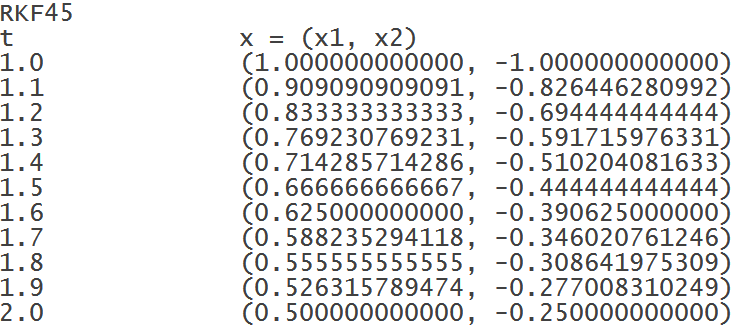
\includegraphics[height=1.75in]{rkf45}
        \caption{RKF45}
    \end{subfigure}%
    ~ 
    \begin{subfigure}[t]{0.5\textwidth}
        \centering
        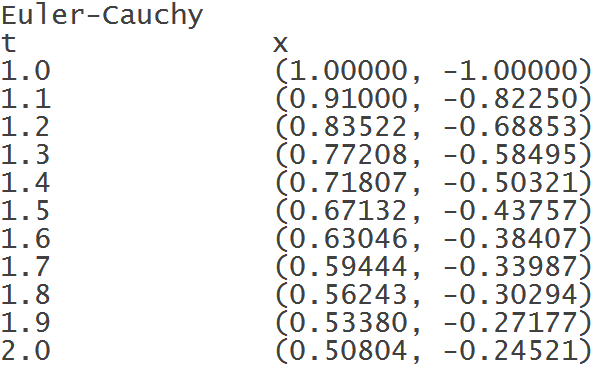
\includegraphics[height=1.75in]{euler_cauchy}
        \caption{Метод Эйлера-Коши}
    \end{subfigure}
    \caption{Вывод программы}
    \label{pic:demo1}
\end{figure} 

На рисунках \ref{pic:graphic1} и \ref{pic:graphic2} изображены графики зависимости нормы матрицы от $\varepsilon$ на всем интервале и на отрезке $[10^{-16}, 10^{-1}]$ соответственно.

\section{Выводы}

\newpage

\section*{Приложение 1. Листинги кода}

\end{document}
